% Created by tikzDevice version 0.12 on 2019-04-27 00:00:34
% !TEX encoding = UTF-8 Unicode
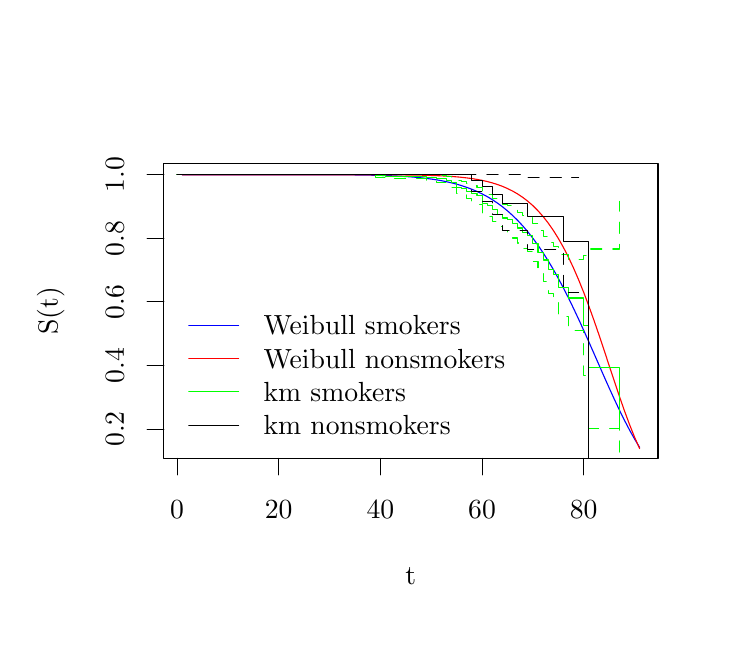
\begin{tikzpicture}[x=1pt,y=1pt]
\definecolor{fillColor}{RGB}{255,255,255}
\path[use as bounding box,fill=fillColor,fill opacity=0.00] (0,0) rectangle (252.94,216.81);
\begin{scope}
\path[clip] ( 49.20, 61.20) rectangle (227.75,167.61);
\definecolor{drawColor}{RGB}{0,0,255}

\path[draw=drawColor,line width= 0.4pt,line join=round,line cap=round] ( 55.81,163.67) --
	( 57.65,163.67) --
	( 59.49,163.67) --
	( 61.32,163.67) --
	( 63.16,163.67) --
	( 65.00,163.67) --
	( 66.83,163.67) --
	( 68.67,163.67) --
	( 70.51,163.67) --
	( 72.34,163.67) --
	( 74.18,163.67) --
	( 76.02,163.67) --
	( 77.86,163.67) --
	( 79.69,163.67) --
	( 81.53,163.67) --
	( 83.37,163.67) --
	( 85.20,163.67) --
	( 87.04,163.67) --
	( 88.88,163.67) --
	( 90.71,163.67) --
	( 92.55,163.67) --
	( 94.39,163.67) --
	( 96.22,163.67) --
	( 98.06,163.67) --
	( 99.90,163.66) --
	(101.73,163.66) --
	(103.57,163.66) --
	(105.41,163.66) --
	(107.25,163.65) --
	(109.08,163.65) --
	(110.92,163.64) --
	(112.76,163.63) --
	(114.59,163.62) --
	(116.43,163.61) --
	(118.27,163.59) --
	(120.10,163.57) --
	(121.94,163.54) --
	(123.78,163.51) --
	(125.61,163.47) --
	(127.45,163.43) --
	(129.29,163.37) --
	(131.12,163.30) --
	(132.96,163.22) --
	(134.80,163.13) --
	(136.64,163.02) --
	(138.47,162.89) --
	(140.31,162.74) --
	(142.15,162.56) --
	(143.98,162.35) --
	(145.82,162.11) --
	(147.66,161.84) --
	(149.49,161.52) --
	(151.33,161.15) --
	(153.17,160.73) --
	(155.00,160.26) --
	(156.84,159.72) --
	(158.68,159.10) --
	(160.52,158.41) --
	(162.35,157.63) --
	(164.19,156.75) --
	(166.03,155.77) --
	(167.86,154.68) --
	(169.70,153.46) --
	(171.54,152.11) --
	(173.37,150.62) --
	(175.21,148.97) --
	(177.05,147.17) --
	(178.88,145.20) --
	(180.72,143.05) --
	(182.56,140.72) --
	(184.39,138.20) --
	(186.23,135.49) --
	(188.07,132.59) --
	(189.91,129.50) --
	(191.74,126.22) --
	(193.58,122.76) --
	(195.42,119.14) --
	(197.25,115.36) --
	(199.09,111.45) --
	(200.93,107.42) --
	(202.76,103.31) --
	(204.60, 99.14) --
	(206.44, 94.95) --
	(208.27, 90.77) --
	(210.11, 86.65) --
	(211.95, 82.62) --
	(213.78, 78.72) --
	(215.62, 74.99) --
	(217.46, 71.46) --
	(219.30, 68.17) --
	(221.13, 65.14);
\end{scope}
\begin{scope}
\path[clip] (  0.00,  0.00) rectangle (252.94,216.81);
\definecolor{drawColor}{RGB}{0,0,0}

\path[draw=drawColor,line width= 0.4pt,line join=round,line cap=round] ( 53.98, 61.20) -- (200.93, 61.20);

\path[draw=drawColor,line width= 0.4pt,line join=round,line cap=round] ( 53.98, 61.20) -- ( 53.98, 55.20);

\path[draw=drawColor,line width= 0.4pt,line join=round,line cap=round] ( 90.71, 61.20) -- ( 90.71, 55.20);

\path[draw=drawColor,line width= 0.4pt,line join=round,line cap=round] (127.45, 61.20) -- (127.45, 55.20);

\path[draw=drawColor,line width= 0.4pt,line join=round,line cap=round] (164.19, 61.20) -- (164.19, 55.20);

\path[draw=drawColor,line width= 0.4pt,line join=round,line cap=round] (200.93, 61.20) -- (200.93, 55.20);

\node[text=drawColor,anchor=base,inner sep=0pt, outer sep=0pt, scale=  1.00] at ( 53.98, 39.60) {0};

\node[text=drawColor,anchor=base,inner sep=0pt, outer sep=0pt, scale=  1.00] at ( 90.71, 39.60) {20};

\node[text=drawColor,anchor=base,inner sep=0pt, outer sep=0pt, scale=  1.00] at (127.45, 39.60) {40};

\node[text=drawColor,anchor=base,inner sep=0pt, outer sep=0pt, scale=  1.00] at (164.19, 39.60) {60};

\node[text=drawColor,anchor=base,inner sep=0pt, outer sep=0pt, scale=  1.00] at (200.93, 39.60) {80};

\path[draw=drawColor,line width= 0.4pt,line join=round,line cap=round] ( 49.20, 71.76) -- ( 49.20,163.67);

\path[draw=drawColor,line width= 0.4pt,line join=round,line cap=round] ( 49.20, 71.76) -- ( 43.20, 71.76);

\path[draw=drawColor,line width= 0.4pt,line join=round,line cap=round] ( 49.20, 94.74) -- ( 43.20, 94.74);

\path[draw=drawColor,line width= 0.4pt,line join=round,line cap=round] ( 49.20,117.71) -- ( 43.20,117.71);

\path[draw=drawColor,line width= 0.4pt,line join=round,line cap=round] ( 49.20,140.69) -- ( 43.20,140.69);

\path[draw=drawColor,line width= 0.4pt,line join=round,line cap=round] ( 49.20,163.67) -- ( 43.20,163.67);

\node[text=drawColor,rotate= 90.00,anchor=base,inner sep=0pt, outer sep=0pt, scale=  1.00] at ( 34.80, 71.76) {0.2};

\node[text=drawColor,rotate= 90.00,anchor=base,inner sep=0pt, outer sep=0pt, scale=  1.00] at ( 34.80, 94.74) {0.4};

\node[text=drawColor,rotate= 90.00,anchor=base,inner sep=0pt, outer sep=0pt, scale=  1.00] at ( 34.80,117.71) {0.6};

\node[text=drawColor,rotate= 90.00,anchor=base,inner sep=0pt, outer sep=0pt, scale=  1.00] at ( 34.80,140.69) {0.8};

\node[text=drawColor,rotate= 90.00,anchor=base,inner sep=0pt, outer sep=0pt, scale=  1.00] at ( 34.80,163.67) {1.0};

\path[draw=drawColor,line width= 0.4pt,line join=round,line cap=round] ( 49.20, 61.20) --
	(227.75, 61.20) --
	(227.75,167.61) --
	( 49.20,167.61) --
	( 49.20, 61.20);
\end{scope}
\begin{scope}
\path[clip] (  0.00,  0.00) rectangle (252.94,216.81);
\definecolor{drawColor}{RGB}{0,0,0}

\node[text=drawColor,anchor=base,inner sep=0pt, outer sep=0pt, scale=  1.00] at (138.47, 15.60) {t};

\node[text=drawColor,rotate= 90.00,anchor=base,inner sep=0pt, outer sep=0pt, scale=  1.00] at ( 10.80,114.41) {S(t)};
\end{scope}
\begin{scope}
\path[clip] ( 49.20, 61.20) rectangle (227.75,167.61);
\definecolor{drawColor}{RGB}{255,0,0}

\path[draw=drawColor,line width= 0.4pt,line join=round,line cap=round] ( 55.81,163.67) --
	( 57.65,163.67) --
	( 59.49,163.67) --
	( 61.32,163.67) --
	( 63.16,163.67) --
	( 65.00,163.67) --
	( 66.83,163.67) --
	( 68.67,163.67) --
	( 70.51,163.67) --
	( 72.34,163.67) --
	( 74.18,163.67) --
	( 76.02,163.67) --
	( 77.86,163.67) --
	( 79.69,163.67) --
	( 81.53,163.67) --
	( 83.37,163.67) --
	( 85.20,163.67) --
	( 87.04,163.67) --
	( 88.88,163.67) --
	( 90.71,163.67) --
	( 92.55,163.67) --
	( 94.39,163.67) --
	( 96.22,163.67) --
	( 98.06,163.67) --
	( 99.90,163.67) --
	(101.73,163.67) --
	(103.57,163.67) --
	(105.41,163.67) --
	(107.25,163.67) --
	(109.08,163.67) --
	(110.92,163.67) --
	(112.76,163.67) --
	(114.59,163.67) --
	(116.43,163.67) --
	(118.27,163.66) --
	(120.10,163.66) --
	(121.94,163.66) --
	(123.78,163.66) --
	(125.61,163.65) --
	(127.45,163.65) --
	(129.29,163.64) --
	(131.12,163.63) --
	(132.96,163.62) --
	(134.80,163.61) --
	(136.64,163.59) --
	(138.47,163.57) --
	(140.31,163.54) --
	(142.15,163.51) --
	(143.98,163.46) --
	(145.82,163.41) --
	(147.66,163.34) --
	(149.49,163.26) --
	(151.33,163.17) --
	(153.17,163.05) --
	(155.00,162.90) --
	(156.84,162.73) --
	(158.68,162.52) --
	(160.52,162.28) --
	(162.35,161.98) --
	(164.19,161.63) --
	(166.03,161.22) --
	(167.86,160.73) --
	(169.70,160.15) --
	(171.54,159.48) --
	(173.37,158.69) --
	(175.21,157.78) --
	(177.05,156.72) --
	(178.88,155.50) --
	(180.72,154.09) --
	(182.56,152.49) --
	(184.39,150.66) --
	(186.23,148.58) --
	(188.07,146.24) --
	(189.91,143.61) --
	(191.74,140.68) --
	(193.58,137.43) --
	(195.42,133.85) --
	(197.25,129.94) --
	(199.09,125.69) --
	(200.93,121.13) --
	(202.76,116.27) --
	(204.60,111.14) --
	(206.44,105.80) --
	(208.27,100.31) --
	(210.11, 94.74) --
	(211.95, 89.17) --
	(213.78, 83.70) --
	(215.62, 78.43) --
	(217.46, 73.45) --
	(219.30, 68.85) --
	(221.13, 64.71);
\definecolor{drawColor}{RGB}{0,255,0}

\path[draw=drawColor,line width= 0.4pt,line join=round,line cap=round] ( 53.98,163.67) --
	(125.61,163.67) --
	(125.61,163.37) --
	(129.29,163.37) --
	(129.29,163.07) --
	(143.98,163.07) --
	(143.98,162.76) --
	(147.66,162.76) --
	(147.66,162.15) --
	(151.33,162.15) --
	(151.33,161.50) --
	(153.17,161.50) --
	(153.17,160.84) --
	(155.00,160.84) --
	(155.00,159.15) --
	(156.84,159.15) --
	(156.84,158.80) --
	(158.68,158.80) --
	(158.68,157.68) --
	(160.52,157.68) --
	(160.52,156.90) --
	(162.35,156.90) --
	(162.35,156.08) --
	(164.19,156.08) --
	(164.19,153.42) --
	(166.03,153.42) --
	(166.03,152.48) --
	(167.86,152.48) --
	(167.86,150.97) --
	(169.70,150.97) --
	(169.70,149.29) --
	(171.54,149.29) --
	(171.54,148.05) --
	(173.37,148.05) --
	(173.37,147.35) --
	(175.21,147.35) --
	(175.21,145.90) --
	(177.05,145.90) --
	(177.05,144.41) --
	(178.88,144.41) --
	(178.88,142.77) --
	(180.72,142.77) --
	(180.72,141.87) --
	(182.56,141.87) --
	(182.56,138.93) --
	(184.39,138.93) --
	(184.39,135.46) --
	(186.23,135.46) --
	(186.23,132.84) --
	(188.07,132.84) --
	(188.07,129.47) --
	(189.91,129.47) --
	(189.91,127.60) --
	(191.74,127.60) --
	(191.74,122.82) --
	(195.42,122.82) --
	(195.42,119.12) --
	(200.93,119.12) --
	(200.93,109.07) --
	(202.76,109.07) --
	(202.76, 94.00) --
	(213.78, 94.00) --
	(213.78, 71.39);

\path[draw=drawColor,line width= 0.4pt,dash pattern=on 4pt off 4pt ,line join=round,line cap=round] ( 53.98,163.67) --
	(125.61,163.67) --
	(125.61,162.79) --
	(129.29,162.79) --
	(129.29,162.25) --
	(143.98,162.25) --
	(143.98,161.75) --
	(147.66,161.75) --
	(147.66,160.83) --
	(151.33,160.83) --
	(151.33,159.91) --
	(153.17,159.91) --
	(153.17,159.03) --
	(155.00,159.03) --
	(155.00,156.84) --
	(156.84,156.84) --
	(156.84,156.40) --
	(158.68,156.40) --
	(158.68,155.01) --
	(160.52,155.01) --
	(160.52,154.05) --
	(162.35,154.05) --
	(162.35,153.04) --
	(164.19,153.04) --
	(164.19,149.82) --
	(166.03,149.82) --
	(166.03,148.69) --
	(167.86,148.69) --
	(167.86,146.89) --
	(169.70,146.89) --
	(169.70,144.88) --
	(171.54,144.88) --
	(171.54,143.38) --
	(173.37,143.38) --
	(173.37,142.54) --
	(175.21,142.54) --
	(175.21,140.79) --
	(177.05,140.79) --
	(177.05,139.00) --
	(178.88,139.00) --
	(178.88,137.04) --
	(180.72,137.04) --
	(180.72,135.95) --
	(182.56,135.95) --
	(182.56,132.41) --
	(184.39,132.41) --
	(184.39,128.22) --
	(186.23,128.22) --
	(186.23,125.06) --
	(188.07,125.06) --
	(188.07,120.90) --
	(189.91,120.90) --
	(189.91,118.58) --
	(191.74,118.58) --
	(191.74,112.56) --
	(195.42,112.56) --
	(195.42,107.54) --
	(200.93,107.54) --
	(200.93, 91.18) --
	(202.76, 91.18) --
	(202.76, 72.00) --
	(213.78, 72.00) --
	(213.78, 53.64);

\path[draw=drawColor,line width= 0.4pt,dash pattern=on 4pt off 4pt ,line join=round,line cap=round] ( 53.98,163.67) --
	(147.66,163.67) --
	(147.66,163.48) --
	(151.33,163.48) --
	(151.33,163.10) --
	(153.17,163.10) --
	(153.17,162.68) --
	(155.00,162.68) --
	(155.00,161.50) --
	(156.84,161.50) --
	(156.84,161.24) --
	(158.68,161.24) --
	(158.68,160.42) --
	(160.52,160.42) --
	(160.52,159.83) --
	(162.35,159.83) --
	(162.35,159.21) --
	(164.19,159.21) --
	(164.19,157.16) --
	(166.03,157.16) --
	(166.03,156.41) --
	(167.86,156.41) --
	(167.86,155.22) --
	(169.70,155.22) --
	(169.70,153.91) --
	(171.54,153.91) --
	(171.54,152.94) --
	(173.37,152.94) --
	(173.37,152.41) --
	(175.21,152.41) --
	(175.21,151.30) --
	(177.05,151.30) --
	(177.05,150.14) --
	(178.88,150.14) --
	(178.88,148.87) --
	(180.72,148.87) --
	(180.72,148.19) --
	(182.56,148.19) --
	(182.56,145.96) --
	(184.39,145.96) --
	(184.39,143.36) --
	(186.23,143.36) --
	(186.23,141.40) --
	(188.07,141.40) --
	(188.07,139.07) --
	(189.91,139.07) --
	(189.91,137.77) --
	(191.74,137.77) --
	(191.74,134.73) --
	(195.42,134.73) --
	(195.42,132.98) --
	(200.93,132.98) --
	(200.93,134.50) --
	(202.76,134.50) --
	(202.76,136.82) --
	(213.78,136.82) --
	(213.78,154.00);
\definecolor{drawColor}{RGB}{0,0,0}

\path[draw=drawColor,line width= 0.4pt,line join=round,line cap=round] ( 53.98,163.67) --
	(160.52,163.67) --
	(160.52,161.62) --
	(164.19,161.62) --
	(164.19,159.45) --
	(167.86,159.45) --
	(167.86,156.68) --
	(171.54,156.68) --
	(171.54,153.20) --
	(180.72,153.20) --
	(180.72,148.66) --
	(193.58,148.66) --
	(193.58,139.58) --
	(202.76,139.58) --
	(202.76, 48.78);

\path[draw=drawColor,line width= 0.4pt,dash pattern=on 4pt off 4pt ,line join=round,line cap=round] ( 53.98,163.67) --
	(160.52,163.67) --
	(160.52,157.70) --
	(164.19,157.70) --
	(164.19,153.85) --
	(167.86,153.85) --
	(167.86,149.20) --
	(171.54,149.20) --
	(171.54,143.61) --
	(180.72,143.61) --
	(180.72,136.49) --
	(193.58,136.49) --
	(193.58,121.10) --
	(199.09,121.10);

\path[draw=drawColor,line width= 0.4pt,dash pattern=on 4pt off 4pt ,line join=round,line cap=round] ( 53.98,163.67) --
	(180.72,163.67) --
	(180.72,162.52) --
	(193.58,162.52) --
	(193.58,162.79) --
	(199.09,162.79);

\path[] ( 49.22,121.21) rectangle (177.06, 61.21);
\definecolor{drawColor}{RGB}{0,0,255}

\path[draw=drawColor,line width= 0.4pt,line join=round,line cap=round] ( 58.22,109.21) -- ( 76.22,109.21);
\definecolor{drawColor}{RGB}{255,0,0}

\path[draw=drawColor,line width= 0.4pt,line join=round,line cap=round] ( 58.22, 97.21) -- ( 76.22, 97.21);
\definecolor{drawColor}{RGB}{0,255,0}

\path[draw=drawColor,line width= 0.4pt,line join=round,line cap=round] ( 58.22, 85.21) -- ( 76.22, 85.21);
\definecolor{drawColor}{RGB}{0,0,0}

\path[draw=drawColor,line width= 0.4pt,line join=round,line cap=round] ( 58.22, 73.21) -- ( 76.22, 73.21);

\node[text=drawColor,anchor=base west,inner sep=0pt, outer sep=0pt, scale=  1.00] at ( 85.22,105.77) {Weibull smokers};

\node[text=drawColor,anchor=base west,inner sep=0pt, outer sep=0pt, scale=  1.00] at ( 85.22, 93.77) {Weibull nonsmokers};

\node[text=drawColor,anchor=base west,inner sep=0pt, outer sep=0pt, scale=  1.00] at ( 85.22, 81.77) {km smokers};

\node[text=drawColor,anchor=base west,inner sep=0pt, outer sep=0pt, scale=  1.00] at ( 85.22, 69.77) {km nonsmokers};
\end{scope}
\end{tikzpicture}
